%%*************************************************************************
%% Legal Notice:
%% This code is offered as-is without any warranty either expressed or
%% implied; without even the implied warranty of MERCHANTABILITY or
%% FITNESS FOR A PARTICULAR PURPOSE! 
%% User assumes all risk.
%% In no event shall the IEEE or any contributor to this code be liable for
%% any damages or losses, including, but not limited to, incidental,
%% consequential, or any other damages, resulting from the use or misuse
%% of any information contained here.
%%
%% All comments are the opinions of their respective authors and are not
%% necessarily endorsed by the IEEE.
%%
%% This work is distributed under the LaTeX Project Public License (LPPL)
%% ( http://www.latex-project.org/ ) version 1.3, and may be freely used,
%% distributed and modified. A copy of the LPPL, version 1.3, is included
%% in the base LaTeX documentation of all distributions of LaTeX released
%% 2003/12/01 or later.
%% Retain all contribution notices and credits.
%% ** Modified files should be clearly indicated as such, including  **
%% ** renaming them and changing author support contact information. **
%%*************************************************************************


% *** Authors should verify (and, if needed, correct) their LaTeX system  ***
% *** with the testflow diagnostic prior to trusting their LaTeX platform ***
% *** with production work. The IEEE's font choices and paper sizes can   ***
% *** trigger bugs that do not appear when using other class files.       ***                          ***
% The testflow support page is at:
% http://www.michaelshell.org/tex/testflow/



\documentclass[conference]{IEEEtran}
% Some Computer Society conferences also require the compsoc mode option,
% but others use the standard conference format.
%
% If IEEEtran.cls has not been installed into the LaTeX system files,
% manually specify the path to it like:
% \documentclass[conference]{../sty/IEEEtran}





% Some very useful LaTeX packages include:
% (uncomment the ones you want to load)


% *** MISC UTILITY PACKAGES ***
%
%\usepackage{ifpdf}
% Heiko Oberdiek's ifpdf.sty is very useful if you need conditional
% compilation based on whether the output is pdf or dvi.
% usage:
% \ifpdf
%   % pdf code
% \else
%   % dvi code
% \fi
% The latest version of ifpdf.sty can be obtained from:
% http://www.ctan.org/pkg/ifpdf
% Also, note that IEEEtran.cls V1.7 and later provides a builtin
% \ifCLASSINFOpdf conditional that works the same way.
% When switching from latex to pdflatex and vice-versa, the compiler may
% have to be run twice to clear warning/error messages.
\usepackage[official]{eurosym}





% *** CITATION PACKAGES ***
%
\usepackage{cite}
% cite.sty was written by Donald Arseneau
% V1.6 and later of IEEEtran pre-defines the format of the cite.sty package
% \cite{} output to follow that of the IEEE. Loading the cite package will
% result in citation numbers being automatically sorted and properly
% "compressed/ranged". e.g., [1], [9], [2], [7], [5], [6] without using
% cite.sty will become [1], [2], [5]--[7], [9] using cite.sty. cite.sty's
% \cite will automatically add leading space, if needed. Use cite.sty's
% noadjust option (cite.sty V3.8 and later) if you want to turn this off
% such as if a citation ever needs to be enclosed in parenthesis.
% cite.sty is already installed on most LaTeX systems. Be sure and use
% version 5.0 (2009-03-20) and later if using hyperref.sty.
% The latest version can be obtained at:
% http://www.ctan.org/pkg/cite
% The documentation is contained in the cite.sty file itself.



% *** GRAPHICS RELATED PACKAGES ***
%
\ifCLASSINFOpdf
\usepackage[pdftex]{graphicx}
  % declare the path(s) where your graphic files are
  % \graphicspath{{../pdf/}{../jpeg/}}
  % and their extensions so you won't have to specify these with
  % every instance of \includegraphics
  % \DeclareGraphicsExtensions{.pdf,.jpeg,.png}
\else
  % or other class option (dvipsone, dvipdf, if not using dvips). graphicx
  % will default to the driver specified in the system graphics.cfg if no
  % driver is specified.
  % \usepackage[dvips]{graphicx}
  % declare the path(s) where your graphic files are
  % \graphicspath{{../eps/}}
  % and their extensions so you won't have to specify these with
  % every instance of \includegraphics
  % \DeclareGraphicsExtensions{.eps}
\fi
% graphicx was written by David Carlisle and Sebastian Rahtz. It is
% required if you want graphics, photos, etc. graphicx.sty is already
% installed on most LaTeX systems. The latest version and documentation
% can be obtained at: 
% http://www.ctan.org/pkg/graphicx
% Another good source of documentation is "Using Imported Graphics in
% LaTeX2e" by Keith Reckdahl which can be found at:
% http://www.ctan.org/pkg/epslatex
%
% latex, and pdflatex in dvi mode, support graphics in encapsulated
% postscript (.eps) format. pdflatex in pdf mode supports graphics
% in .pdf, .jpeg, .png and .mps (metapost) formats. Users should ensure
% that all non-photo figures use a vector format (.eps, .pdf, .mps) and
% not a bitmapped formats (.jpeg, .png). The IEEE frowns on bitmapped formats
% which can result in "jaggedy"/blurry rendering of lines and letters as
% well as large increases in file sizes.
%
% You can find documentation about the pdfTeX application at:
% http://www.tug.org/applications/pdftex





% *** MATH PACKAGES ***
%
%\usepackage{amsmath}
% A popular package from the American Mathematical Society that provides
% many useful and powerful commands for dealing with mathematics.
%
% Note that the amsmath package sets \interdisplaylinepenalty to 10000
% thus preventing page breaks from occurring within multiline equations. Use:
%\interdisplaylinepenalty=2500
% after loading amsmath to restore such page breaks as IEEEtran.cls normally
% does. amsmath.sty is already installed on most LaTeX systems. The latest
% version and documentation can be obtained at:
% http://www.ctan.org/pkg/amsmath





% *** SPECIALIZED LIST PACKAGES ***
%
%\usepackage{algorithmic}
% algorithmic.sty was written by Peter Williams and Rogerio Brito.
% This package provides an algorithmic environment fo describing algorithms.
% You can use the algorithmic environment in-text or within a figure
% environment to provide for a floating algorithm. Do NOT use the algorithm
% floating environment provided by algorithm.sty (by the same authors) or
% algorithm2e.sty (by Christophe Fiorio) as the IEEE does not use dedicated
% algorithm float types and packages that provide these will not provide
% correct IEEE style captions. The latest version and documentation of
% algorithmic.sty can be obtained at:
% http://www.ctan.org/pkg/algorithms
% Also of interest may be the (relatively newer and more customizable)
% algorithmicx.sty package by Szasz Janos:
% http://www.ctan.org/pkg/algorithmicx




% *** ALIGNMENT PACKAGES ***
%
%\usepackage{array}
% Frank Mittelbach's and David Carlisle's array.sty patches and improves
% the standard LaTeX2e array and tabular environments to provide better
% appearance and additional user controls. As the default LaTeX2e table
% generation code is lacking to the point of almost being broken with
% respect to the quality of the end results, all users are strongly
% advised to use an enhanced (at the very least that provided by array.sty)
% set of table tools. array.sty is already installed on most systems. The
% latest version and documentation can be obtained at:
% http://www.ctan.org/pkg/array


% IEEEtran contains the IEEEeqnarray family of commands that can be used to
% generate multiline equations as well as matrices, tables, etc., of high
% quality.




% *** SUBFIGURE PACKAGES ***
%\ifCLASSOPTIONcompsoc
%  \usepackage[caption=false,font=normalsize,labelfont=sf,textfont=sf]{subfig}
%\else
%  \usepackage[caption=false,font=footnotesize]{subfig}
%\fi
% subfig.sty, written by Steven Douglas Cochran, is the modern replacement
% for subfigure.sty, the latter of which is no longer maintained and is
% incompatible with some LaTeX packages including fixltx2e. However,
% subfig.sty requires and automatically loads Axel Sommerfeldt's caption.sty
% which will override IEEEtran.cls' handling of captions and this will result
% in non-IEEE style figure/table captions. To prevent this problem, be sure
% and invoke subfig.sty's "caption=false" package option (available since
% subfig.sty version 1.3, 2005/06/28) as this is will preserve IEEEtran.cls
% handling of captions.
% Note that the Computer Society format requires a larger sans serif font
% than the serif footnote size font used in traditional IEEE formatting
% and thus the need to invoke different subfig.sty package options depending
% on whether compsoc mode has been enabled.
%
% The latest version and documentation of subfig.sty can be obtained at:
% http://www.ctan.org/pkg/subfig




% *** FLOAT PACKAGES ***
%
%\usepackage{fixltx2e}
% fixltx2e, the successor to the earlier fix2col.sty, was written by
% Frank Mittelbach and David Carlisle. This package corrects a few problems
% in the LaTeX2e kernel, the most notable of which is that in current
% LaTeX2e releases, the ordering of single and double column floats is not
% guaranteed to be preserved. Thus, an unpatched LaTeX2e can allow a
% single column figure to be placed prior to an earlier double column
% figure.
% Be aware that LaTeX2e kernels dated 2015 and later have fixltx2e.sty's
% corrections already built into the system in which case a warning will
% be issued if an attempt is made to load fixltx2e.sty as it is no longer
% needed.
% The latest version and documentation can be found at:
% http://www.ctan.org/pkg/fixltx2e


%\usepackage{stfloats}
% stfloats.sty was written by Sigitas Tolusis. This package gives LaTeX2e
% the ability to do double column floats at the bottom of the page as well
% as the top. (e.g., "\begin{figure*}[!b]" is not normally possible in
% LaTeX2e). It also provides a command:
%\fnbelowfloat
% to enable the placement of footnotes below bottom floats (the standard
% LaTeX2e kernel puts them above bottom floats). This is an invasive package
% which rewrites many portions of the LaTeX2e float routines. It may not work
% with other packages that modify the LaTeX2e float routines. The latest
% version and documentation can be obtained at:
% http://www.ctan.org/pkg/stfloats
% Do not use the stfloats baselinefloat ability as the IEEE does not allow
% \baselineskip to stretch. Authors submitting work to the IEEE should note
% that the IEEE rarely uses double column equations and that authors should try
% to avoid such use. Do not be tempted to use the cuted.sty or midfloat.sty
% packages (also by Sigitas Tolusis) as the IEEE does not format its papers in
% such ways.
% Do not attempt to use stfloats with fixltx2e as they are incompatible.
% Instead, use Morten Hogholm'a dblfloatfix which combines the features
% of both fixltx2e and stfloats:
%
% \usepackage{dblfloatfix}
% The latest version can be found at:
% http://www.ctan.org/pkg/dblfloatfix




% *** PDF, URL AND HYPERLINK PACKAGES ***
%
%\usepackage{url}
% url.sty was written by Donald Arseneau. It provides better support for
% handling and breaking URLs. url.sty is already installed on most LaTeX
% systems. The latest version and documentation can be obtained at:
% http://www.ctan.org/pkg/url
% Basically, \url{my_url_here}.




% *** Do not adjust lengths that control margins, column widths, etc. ***
% *** Do not use packages that alter fonts (such as pslatex).         ***
% There should be no need to do such things with IEEEtran.cls V1.6 and later.
% (Unless specifically asked to do so by the journal or conference you plan
% to submit to, of course. )


% correct bad hyphenation here
\hyphenation{op-tical net-works semi-conduc-tor}


\begin{document}
%
% paper title
% Titles are generally capitalized except for words such as a, an, and, as,
% at, but, by, for, in, nor, of, on, or, the, to and up, which are usually
% not capitalized unless they are the first or last word of the title.
% Linebreaks \\ can be used within to get better formatting as desired.
% Do not put math or special symbols in the title.
\title{WSN for Cattle Monitoring -- Related Work and Design Proposal}

% author names and affiliations
% use a multiple column layout for up to three different
% affiliations
\author{\IEEEauthorblockN{
Herman Lundkvist\IEEEauthorrefmark{1},
Attila Para\IEEEauthorrefmark{2},
Vipul Mahawar\IEEEauthorrefmark{3} and
Omar Elshal\IEEEauthorrefmark{4}}
\IEEEauthorblockA{\IEEEauthorrefmark{1}Student Id: 0973534\\
Email: h.e.lundkvist@student.tue.nl}
\IEEEauthorblockA{\IEEEauthorrefmark{2}Student Id: 0975194\\
Email: a.para@student.tue.nl}
\IEEEauthorblockA{\IEEEauthorrefmark{3}Student Id: 0980015\\
Email: v.mahawar@student.tue.nl}
\IEEEauthorblockA{\IEEEauthorrefmark{4}Student Id: 0980295\\
Email: o.a.m.elshal@student.tue.nl}}

% conference papers do not typically use \thanks and this command
% is locked out in conference mode. If really needed, such as for
% the acknowledgment of grants, issue a \IEEEoverridecommandlockouts
% after \documentclass

% for over three affiliations, or if they all won't fit within the width
% of the page, use this alternative format:
% 
%\author{\IEEEauthorblockN{Michael Shell\IEEEauthorrefmark{1},
%Homer Simpson\IEEEauthorrefmark{2},
%James Kirk\IEEEauthorrefmark{3}, 
%Montgomery Scott\IEEEauthorrefmark{3} and
%Eldon Tyrell\IEEEauthorrefmark{4}}
%\IEEEauthorblockA{\IEEEauthorrefmark{1}School of Electrical and Computer Engineering\\
%Georgia Institute of Technology,
%Atlanta, Georgia 30332--0250\\ Email: see http://www.michaelshell.org/contact.html}
%\IEEEauthorblockA{\IEEEauthorrefmark{2}Twentieth Century Fox, Springfield, USA\\
%Email: homer@thesimpsons.com}
%\IEEEauthorblockA{\IEEEauthorrefmark{3}Starfleet Academy, San Francisco, California 96678-2391\\
%Telephone: (800) 555--1212, Fax: (888) 555--1212}
%\IEEEauthorblockA{\IEEEauthorrefmark{4}Tyrell Inc., 123 Replicant Street, Los Angeles, California 90210--4321}}




% use for special paper notices
%\IEEEspecialpapernotice{(Invited Paper)}




% make the title area
\maketitle

% For peer review papers, you can put extra information on the cover
% page as needed:
% \ifCLASSOPTIONpeerreview
% \begin{center} \bfseries EDICS Category: 3-BBND \end{center}
% \fi
%
% For peerreview papers, this IEEEtran command inserts a page break and
% creates the second title. It will be ignored for other modes.
\IEEEpeerreviewmaketitle


\section{Introduction}

\subsection{Background}

The livestock industry constitutes a considerable part of the world’s economy.
In fact, it generates around \euro{} 8.6 billion every year in the Netherlands
alone~\cite{nedgov}. At the same time, there is a clear trend of automation in
this sector that aims to increase the efficiency and decrease the amount of
human labour.

However, one of the major costs for the farmers in this field is due to the
diseases contracted by their animals. By developing a system that could detect
such diseases, and other abnormal behavior, one could potentially reduce this
cost by a great amount.  


\subsection{Application Description}

The main purpose of this project is to design a system that can help farmers
monitor the health of cattle while they are grazing. This will be done using
wireless sensor network (WSN) technology, because of its ability to deliver
real-time monitoring at a very low cost.  However, on account of range
limitations of WSN transceivers, the system will be designed for a relatively
small field of 10 ha which is in the range of an average dairy farm in the
Netherlands~\cite{agriculturalsystems}.

The network of the system will consist of three types of nodes: a base station,
which acts as a data sink; sensor nodes, one for each head of cattle, recording
health characteristics; and a number of relay nodes on fixed positions in the
field, forwarding data from the sensor nodes to the base station. The reason
for using relay nodes, is to be able to cover the majority of the field.

The system will be used both to detect different types of diseases, for
example: fever, lameness and mastitis, and to detect if a cow is in estrus.
This can be accomplished by the of use accelerometer-, microphone-, and
temperature sensors in the sensor nodes~\cite{hese2014}. Every 5 minutes, the
sensor nodes will send the acquired data in a processed form to the base
station for storage. The base station can analyse the sample values to detect
patterns that correspond to different diseases or the onset of estrus.

\subsection{Related Work}

Wireless livestock monitoring has became a widely researched area in recent
years due to the increased availability and lower costs of wireless sensor
network technologies. WSN have been utilized in many livestock monitoring
applications around the world such as animal localization, behavior analysis,
health monitoring or pregnancy detection in cows. Several studies are
concentrated to raw data collection~\cite{GU06AN,WA15IN} for later data
processing and research. The main drawback of these studies is the high energy
consumption of the sensor nodes, which limits the lifetime of the nodes to only
a few days at most.  Also the storage and processing of collected data would be
a problem in longer term.

Most of the livestock monitoring WSNs are designed for cattles \cite{GU06AN,
KU15AZ, SM06AN, SO05AW, MA14CA, HW11DE, WA15IN, KW12PR, PA15SO, NO13WI, HU10ZI,
KW09WI} but there are also examples of studies for sheep health and behavior
monitoring~\cite{NA12MO} and chicken monitoring for avian influenza
surveillance in poultry farms with ultra low power wireless sensor
nodes~\cite{OK12DE, OK13DE}. The wireless health monitoring of cows has been
one of the most important researched topic among authors. Kumar et
al.~\cite{KU15AZ} and Wang et al.~\cite{WA15IN} both developed cattle health
monitoring WSNs based on the IEEE~802.15.4 protocol. Hwang et al.~\cite{HW11DE}
showed that continuous monitoring and comparison of cattle activity can be used
for disease prediction and prevention. In addition to disease prediction,
pregnancy detection is also possible using continuous monitoring~\cite{NO13WI}.

Wireless sensor networks can be used for livestock localization
indoor~\cite{AS13WI} or outdoor~\cite{PA15SO, HU10ZI}. Panckhurst et
al.~\cite{PA15SO} developed a GPS based wireless positioning system, while
Huircan et al.~\cite{HU10ZI} demonstrated that the link quality indication
(LQI) feature of the ZigBee protocol can also be a candidate for outdoor
livestock localization. Livestock positioning can have different purposes
around the world, like the prevention of pastureland degradation and
desertification in Mongolia~\cite{CH13CL} or cattle rustling prevention in
Africa~\cite{MA14CA}.

The ZigBee protocol and a carrier frequency of 2.4 GHz are widely used
\cite{KU15AZ, MA14CA, HU10ZI, NA12MO}, however some of the authors
\cite{SO05AW, OK12DE, OK13DE, PA15SO} prefered sub-gigahertz carrier
frequencies due to the higher communication distance. Sousa Silva et
al.~\cite{SO05AW} have demonstrated that a Floating Base Sensor Network (FBSN)
is also a feasible solution for data collection in large mobile wireless sensor
networks. Kwong et al.~\cite{KW09WI} have analysed the problem of signal
penetration through animal's body and they proposed a two antennae scheme for
an optimized radio coverage of the cattle's neck collar. In this project we
will not consider the interference caused by the body of the cows.

\section{Application Specific Challenges}

\subsection{Mobility}

Mobility presents a major challenge for sensor nodes mounted on cattle since
they are subject to frequent changes in location.  The animal monitoring system
must be able to support animal mobility. The network topology and routing paths
should therefore be dynamic, able to respond to frequent animal movement while
optimising packet delivery.

\subsection{Size of Field}

A key challenge in a wireless network of this kind is the coverage of the
wireless nodes. In cattle monitoring WSNs the network architecture should be
able to cover enough area of the fields and must be scalable accordingly when
needed for larger fields. The average size of a dairy farm field in the
Netherlands is around 100,000 m$^2$ and the maximum range of Zigbee WSN
protocol is approximately 500 m, so theoretically, only one or two relay nodes
could cover a sufficient area of the field. In reality, transceivers with such
range capabilities are not used in WSN applications, because of cost and power
constraints. 

\subsection{Wireless Communication}

As the animals move freely on the field, wireless technology is considered the
only feasible method to establish and maintain communication between a base
station and network nodes attached to the cattle. The wireless communication
imposes several challenges on the design, like signal attenuation in the
medium, interference from other radio signals, crosstalk from the other nodes,
etc. As the radio signal generated from the node is weak owing to preserve
battery on the node, a significant amount of wireless signal is attenuated by
the animal tissue.  For maximum signal coverage from relay node the antenna on
the animal is placed on a neck collar with two antenna on both sides of the
neck to have spatial diversity. Also the radio element is switched off as soon
as the data transmission is finished so as to maximize battery life.

\subsection{Energy Consumption}

The battery usage is one of the major constraint in cattle monitoring networks
because the radio collars used for cattle monitoring are expected to run for up
to several years without battery replacement. As there is limited battery power
available per node, low powered, lightweight radio antennas should be
considered for the design. The network protocol should be designed so as to use
limited battery power and only communicate with the base station, to provide
adequate amount of data required for monitoring health of cattle. The
processors used by the nodes should be chosen so as to consume a minimum amount
of power, while still being able to perform the necessary operations on the
data as required by the application.

\subsection{Cost of the System}

The design of a WSN should not be too expensive. Furthermore the wireless nodes
must be low-cost with high lifespan and low maintenance in order to reduce the
cost of managing the system. Another reason for the sensor nodes to be low-cost
is the potentially high number of nodes needed for monitoring an entire herd.

\section{Requirements}

To ensure that the designed system can meet the challenges described in chapter II, it
needs to meet the following requirements:

\begin{enumerate} 

    \item The network must be implemented in such a way that if a sensor node
        moves out of coverage, the sensor node will be reassigned to the
        network once it moves into coverage again.  
        
    \item The end-to-end latency between the sensor nodes and the base station
        must be less than 1 minute for at least 90 \% of data packets.
        
    \item For every sensor node at least 70 \% of the recorded sensor data must
        be delivered to the base station during a 5 hour period.
        
    \item The time until the first sensor node of the network fails must be
        greater than one year.  
        
    \item The network must function and be scalable for up to 100 sensor nodes.
        
    \item The network must continue to function whether nodes are added or
        removed.
    
    \item When out of coverage, each sensor node must be able to store sensor
        values for a period of up to four hours.
    
    \item  On average, 99 \% of the sensor nodes must not be out of coverage
        for more than four hours at a time.

\end{enumerate}


\subsection{Data size}

One of the most important requirements for the system is to be able to handle
the amount of data generated by the sensors. Estimating this amount is thus
also very important. For storing the temperature of the cow after processing
the raw data from the sensors, one byte is enough to give a reasonable
resolution. This is because a dairy cow’s normal rectal temperature lies
between 38.3$^\circ$C and 38.9$^\circ$C~\cite{wikibov} and one could limit the
byte to represent values between 30$^\circ$C and 50$^\circ$C without losing any
information.  Using the same argumentation, one byte could also be used to
store the average heart rate, because the normal heart rate for a dairy cow
lies between 40 and 84 beats per minute~\cite{wikibov}.

In addition, to store the data gathered from the accelerometers, one could
devise a similar strategy to the one used in a study where the behaviour of
sows were classified~\cite{marchiorosows2011}. In this study, the activities
of the animals were organized into four different sets, using a method
specifically developed for low powered embedded devices. This resulted in
a classification with an accuracy of close to 90 \%. Using data in this format,
the researchers were able to detect the onset of farrowing. In this study only
four sets of behaviours were used, if it is possible to develop similar sets
for behavioural studies on cows, one could potentially store this data using
only two bits per sample.

Using two samples for both the temperature and the heart rate, while also
rounding up to the nearest byte, the total amount of sensor data needed to be
sent each five minute interval would be five bytes.


\section{Implementation}

CHANGE THIS

The system will be developed for platforms supporting ContikiOs. For the
physical- and MAC layers, the standard protocol IEEE 802.15.4~\cite{ieee802154}
will be used.  For the network- and application layer, features from ContikiOs
will be used.  Moreover, a routing algorithm might possibly be designed, if the
routing algorithms present in ContikiOs are deemed unfitting for our
application. 

\subsection{Simulation Software}

The design of the network will only be tested in simulation, no real world
experiments will be done. We will use cooja, which is a simulator for contiki
node. This simulator is compatible with the following platforms: TI MSP430x (TI
CC2420), TI MSP430x (TI CC2520), Atmel AVR (TI CC2420), TI MSP430 (TI CC2420)
and TI MSP430 (RFM TR1001).

The number of nodes that can be simulated using this software depends on memory
of the machine running the simulation and the application running on the nodes.
As there is a main simulation thread, using more than two cores (one for the
simulation and one for the rest) gives no significant
improvement~\cite{contikidev}.

To simulate the movement of the cows in Cooja, a mobility plugin first has to
be installed. However, to be able to generate our own specific mobility file,
another tool like BonnMotion has to be used to make the mobility output format
compatible with Cooja’s mobility plugin format. We will only be considering
a few simple mobility models like: the gauss-markov-, the random waypoint- and
the reference point group mobility models. Simulating more complex and accurate
mobility patterns of the cows is not the goal of this project.

To provide a reliable transmission range, there is a UDGM (Unit Disk Graph
Radio Medium) implementation that can be configured to change some parameters
like transmission range and interference range. Depending on the transmission
power parameter, the resulting transmission range will
differ~\cite{contikidev}.

Contiki supports different MAC layers: X-MAC, LLP (Low Power Probing), Simple
TDMA and nullmac (non-persistent CSMA).  X-MAC and LPP are low power MACs that
work best under low traffic loads~\cite{coojacrash}.  Furthermore, Contiki
supports different protocol stacks like uIP which is a very small and fully
compliant TCP/IP stack. Contiki also supports Rime stack which consists of
small layers built on top of each other and has single and multi-hop
broadcast~\cite{coojacrash}.
\subsection{Network Topology}

\begin{figure}
    \centering
    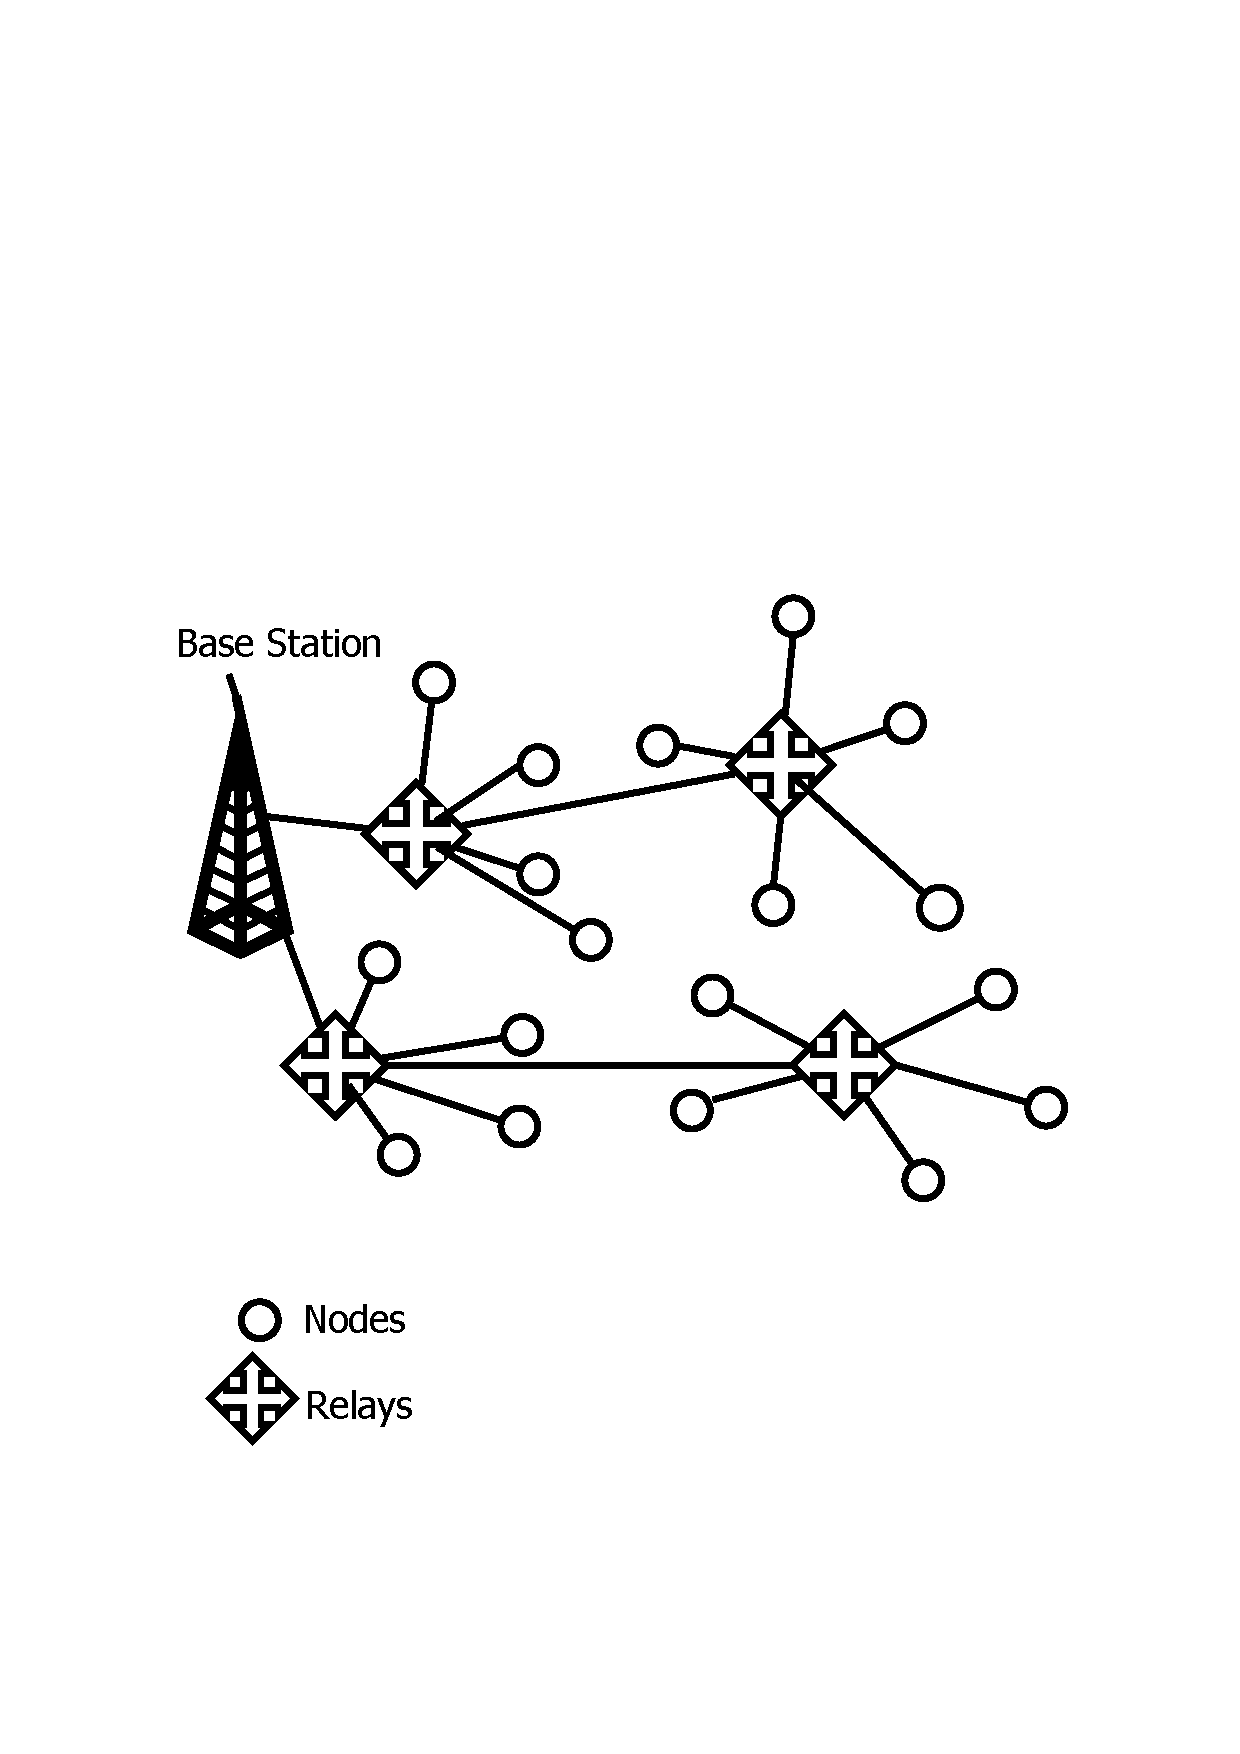
\includegraphics[trim= 0 150  0 150, clip, width=0.4\textwidth]{Figure1.pdf}
    \caption{An overview of the network topology.}
    \label{fig:topology}
\end{figure}

The network topology of the implementation has a tree like structure with
the base station acting as the root of the tree, see Fig \ref{fig:topology}.
The relay nodes act as the branches of the tree, being connected to the base
station through each other, while the sensor nodes behave like the leaves of
the tree.

The sensor nodes send data to any relay node that is within transmission range.
Once received by a relay node, the data will be forwarded to the base station
with the help of a routing protocol.

\subsection{Physical Layer}

In order to get an increased range and mitigate the problems with coverage,
carrier frequencies between 902 MHz and 928 MHz of the IEEE 802.15.4 standard,
were originally considered. However, as these frequencies are not supported by
the TI CC2420 transceiver of the Telos B, a frequency of around 2.4 GHz was
used instead.

For the modulation, the direct-sequence spread spectrum is used, because it is
implemented in the transceiver mentioned above.

Different transmission powers are used for the different node types used in the
implementation. The base station and relay nodes both use the maximum
transmission power of the transceiver to ensure that the relay nodes can be
placed as far apart as possible.  The sensor nodes, on the other hand, use half
of the maximum transmission power to save energy. Because the sensitivity of
the Telos B nodes cannot be changed, this introduces an asymmetry between the
nodes: relay nodes can reach the sensor nodes at maximum range while the
converse is not possible.  Even though this reduces the coverage compared to
the case where maximum transmission power is also used in the sensor nodes,
there is still one benefit: few relay nodes are needed to create a chain to
a relay node placed far away from the base station (for example in a remote
corner of the field). Thus the sensor nodes will still have a short distance to
the nearest relay node.

According to an experiment performed in an outdoor environment, the average
propagation path loss at 60 m for a link between two Telos B Nodes was
estimated to be 92.3 dB. Using this value, along with 0 dBm, the maximum
transmission power of the Telos B node, in the path propagation loss formula:

\begin{displaymath}
    P_{r}[dBm] = P_{t}[dBm] - P_{L}[dB]
\end{displaymath}

where $P_{r}$ is the received power, $P_{t}$ is the transmitted power, and
$P_{L}$ is the propagation path loss gives -92.3 dBm which is greater than -94
dBm, the nominal receiving sensitivity of a Telos B node. Taking this into
account, the maximum transmission distance of the nodes are set to 60 m in the
simulation.

\subsection{MAC Layer}

For the MAC layer, there are two modes to be used in the IEEE 802.15.4
standard: nonbeacon-enabled mode and beacon-enabled mode. In the former
a unslotted CSMA/CA mechanism is used. In the latter one, a more elaborate
scheme is used, wherein special nodes of the network, called coordinators,
regularly send out beacons to synchronize with the nodes they are associated
with. The period between two beacons is called a superframe, and within this
the nodes use a slotted CSMA/CA mechanism.

Because of the need for synchronization, the beacon-enabled mode might cause
problems if a sensor node moves out of the coverage of a coordinator for
a longer period of time, or if a sensor node needs to switch to a different
coordinator.  The sensor node might have to listen for a very long time to
receive the next beacon, possibly even the whole time while it is out of range,
thus consuming a lot of power.

On the other hand, the unslotted CSMA/CA mechanism of the nonbeacon-enabled
mode, in addition to being less complex, does not require the nodes associated
with a coordinator to regularly receive a beacon, and is thus suitable for the
mobile nature of our application. The main drawback is the power consumption
required for continuously listening at regular intervals.  However, since the
relay nodes and the base station are the only ones that need to receive data,
only these will have to listen continuously, and not the sensor nodes. In view
of these arguments, the design will use the nonbeacon-enabled mode. However, as
contiki does not implement unslotted CSMA/CA, we will use one of the
congestion-based MAC layers that contiki provides, in its place.

\subsection{Network Layer}

\section{Performance Evaluation}

\subsection{Mobility Models}

\subsection{Test Scenarios}

\subsection{Data Extraction} 

\subsection{Results}

\subsection{Discussion}

\section{Conclusion}

\section{Future Work}

%\section{Work Plan}

% An example of a floating figure using the graphicx package.
% Note that \label must occur AFTER (or within) \caption.
% For figures, \caption should occur after the \includegraphics.
% Note that IEEEtran v1.7 and later has special internal code that
% is designed to preserve the operation of \label within \caption
% even when the captionsoff option is in effect. However, because
% of issues like this, it may be the safest practice to put all your
% \label just after \caption rather than within \caption{}.
%
% Reminder: the "draftcls" or "draftclsnofoot", not "draft", class
% option should be used if it is desired that the figures are to be
% displayed while in draft mode.
%
%\begin{figure}[!t]
%\centering
%\includegraphics[width=2.5in]{myfigure}
% where an .eps filename suffix will be assumed under latex, 
% and a .pdf suffix will be assumed for pdflatex; or what has been declared
% via \DeclareGraphicsExtensions.
%\caption{Simulation results for the network.}
%\label{fig_sim}
%\end{figure}

% Note that the IEEE typically puts floats only at the top, even when this
% results in a large percentage of a column being occupied by floats.


% An example of a double column floating figure using two subfigures.
% (The subfig.sty package must be loaded for this to work.)
% The subfigure \label commands are set within each subfloat command,
% and the \label for the overall figure must come after \caption.
% \hfil is used as a separator to get equal spacing.
% Watch out that the combined width of all the subfigures on a 
% line do not exceed the text width or a line break will occur.
%
%\begin{figure*}[!t]
%\centering
%\subfloat[Case I]{\includegraphics[width=2.5in]{box}%
%\label{fig_first_case}}
%\hfil
%\subfloat[Case II]{\includegraphics[width=2.5in]{box}%
%\label{fig_second_case}}
%\caption{Simulation results for the network.}
%\label{fig_sim}
%\end{figure*}
%
% Note that often IEEE papers with subfigures do not employ subfigure
% captions (using the optional argument to \subfloat[]), but instead will
% reference/describe all of them (a), (b), etc., within the main caption.
% Be aware that for subfig.sty to generate the (a), (b), etc., subfigure
% labels, the optional argument to \subfloat must be present. If a
% subcaption is not desired, just leave its contents blank,
% e.g., \subfloat[].


% An example of a floating table. Note that, for IEEE style tables, the
% \caption command should come BEFORE the table and, given that table
% captions serve much like titles, are usually capitalized except for words
% such as a, an, and, as, at, but, by, for, in, nor, of, on, or, the, to
% and up, which are usually not capitalized unless they are the first or
% last word of the caption. Table text will default to \footnotesize as
% the IEEE normally uses this smaller font for tables.
% The \label must come after \caption as always.
%
%\begin{table}[!t]
%% increase table row spacing, adjust to taste
%\renewcommand{\arraystretch}{1.3}
% if using array.sty, it might be a good idea to tweak the value of
% \extrarowheight as needed to properly center the text within the cells
%\caption{An Example of a Table}
%\label{table_example}
%\centering
%% Some packages, such as MDW tools, offer better commands for making tables
%% than the plain LaTeX2e tabular which is used here.
%\begin{tabular}{|c||c|}
%\hline
%One & Two\\
%\hline
%Three & Four\\
%\hline
%\end{tabular}
%\end{table}


% Note that the IEEE does not put floats in the very first column
% - or typically anywhere on the first page for that matter. Also,
% in-text middle ("here") positioning is typically not used, but it
% is allowed and encouraged for Computer Society conferences (but
% not Computer Society journals). Most IEEE journals/conferences use
% top floats exclusively. 
% Note that, LaTeX2e, unlike IEEE journals/conferences, places
% footnotes above bottom floats. This can be corrected via the
% \fnbelowfloat command of the stfloats package.


% conference papers do not normally have an appendix

% trigger a \newpage just before the given reference
% number - used to balance the columns on the last page
% adjust value as needed - may need to be readjusted if
% the document is modified later
%\IEEEtriggeratref{8}
% The "triggered" command can be changed if desired:
%\IEEEtriggercmd{\enlargethispage{-5in}}

% references section

% can use a bibliography generated by BibTeX as a .bbl file
% BibTeX documentation can be easily obtained at:
% http://mirror.ctan.org/biblio/bibtex/contrib/doc/
% The IEEEtran BibTeX style support page is at:
% http://www.michaelshell.org/tex/ieeetran/bibtex/
%\bibliographystyle{IEEEtran}
% argument is your BibTeX string definitions and bibliography database(s)
%\bibliography{IEEEabrv,../bib/paper}
%
% <OR> manually copy in the resultant .bbl file
% set second argument of \begin to the number of references
% (used to reserve space for the reference number labels box)
\begin{thebibliography}{1}

\bibitem{nedgov}
    https://www.government.nl/topics/agriculture-and-livestock/contents/livestock-farming,
    taken 12:30 22 sep 2015.

\bibitem{agriculturalsystems}
    D. B. Grigg, \emph{The Agricultural Systems of
    the World: An Evolutionary Approach}, Cambridge University Press, november
    1974, p. 188.

\bibitem{hese2014}
A. ~Helwatkar, D. ~Riordan and J. ~Walsh,
\emph{Sensor Technology For Animal Health Monitoring},
Proceedings of the 8th International Conference on Sensing Technology,
sep, 2014.

\bibitem{GU06AN}
Y. Guo, P. Corke, G. Poulton, T. Wark, G. Bishop-Hurley, and D. Swain, \emph{Animal Behaviour Understanding using Wireless Sensor Networks,} in Proceedings 2006 31st IEEE Conference on Local Computer Networks, 2006, pp. 607–614.

\bibitem{SM06AN}
K. Smith, A. Martinez, R. Craddolph, H. Erickson, D. Andresen, and S. Warren, \emph{An Integrated Cattle Health Monitoring System,} in 28th Annual International Conference of the IEEE Engineering in Medicine and Biology Society, 2006. EMBS ’06, 2006, pp. 4659–4662.

\bibitem{SO05AW}
A. C. de Sousa Silva, A. I. C. Arce, S. Souto, and E. J. X. Costa, \emph{A wireless floating base sensor network for physiological responses of livestock,} Computers and Electronics in Agriculture, vol. 49, no. 2, pp. 246–254, Nov. 2005.

\bibitem{KU15AZ}
A. Kumar and G. P. Hancke, \emph{A Zigbee-Based Animal Health Monitoring System,} IEEE Sensors Journal, vol. 15, no. 1, pp. 610–617, Jan. 2015.

\bibitem{MA14CA}
P. K. Mashoko Nkwari, S. Rimer, and B. S. Paul, \emph{Cattle monitoring system using wireless sensor network in order to prevent cattle rustling,} in IST-Africa Conference Proceedings, 2014, 2014, pp. 1–10.

\bibitem{HW11DE}
J. Hwang and H. Yoe, \emph{Design and implementation of wireless sensor network based livestock activity monitoring system,} in Future Generation Information Technology, Springer, 2011, pp. 161–168.

\bibitem{WA15IN}
H. Wang, B. Davies, and A. O. Fapojuwo, \emph{Inter-wireless body area network scheduling algorithm for livestock health monitoring,} in 2015 IEEE Wireless Communications and Networking Conference (WCNC), 2015, pp. 2132–2137.

\bibitem{KW12PR}
K. H. Kwong, T.-T. Wu, H. G. Goh, K. Sasloglou, B. Stephen, I. Glover, C. Shen, W. Du, C. Michie, and I. Andonovic, \emph{Practical considerations for wireless sensor networks in cattle monitoring applications,} Computers and Electronics in Agriculture, vol. 81, pp. 33–44, Feb. 2012.

\bibitem{PA15SO}
B. Panckhurst, P. Brown, K. Payne, and T. C. A. Molteno, \emph{Solar-powered sensor for continuous monitoring of livestock position,} in 2015 IEEE Sensors Applications Symposium (SAS), 2015, pp. 1–6.

\bibitem{NO13WI}
A. H. H. Nograles and F. S. Caluyo, \emph{Wireless system for pregnancy detection in cows by monitoring temperature changes in body,} in 2013 IEEE 9th International Colloquium on Signal Processing and its Applications (CSPA), 2013, pp. 11–16.

\bibitem{HU10ZI}
J. I. Huircán, C. Muñoz, H. Young, L. Von Dossow, J. Bustos, G. Vivallo, and M. Toneatti, \emph{ZigBee-based wireless sensor network localization for cattle monitoring in grazing fields,} Computers and Electronics in Agriculture, vol. 74, no. 2, pp. 258–264, Nov. 2010.

\bibitem{KW09WI}
K. H. Kwong, T. T. Wu, H. G. Goh, B. Stephen, M. Gilroy, C. Michie, and I. Andonovic, \emph{Wireless sensor networks in agriculture: cattle monitoring for farming industries,} in Progress In Electromagnetics Research Symposium, 2009, vol. 5, pp. 31–35.

\bibitem{CH13CL}
S.-G. Choi, E. Norinpel, and J. Yoo, \emph{Cluster-based routing protocol in wireless sensor networks for tracking livestock movements in Mongolian nomadic herding,} in 2013 8th International Forum on Strategic Technology (IFOST), 2013, vol. 2, pp. 163–167.

\bibitem{OK12DE}
H. Okada, H. Nogami, T. Itoh, and T. Masuda, \emph{Development of Low Power Technologies for Health Monitoring System Using Wireless Sensor Nodes,} in 2012 Second Workshop on Design, Control and Software Implementation for Distributed MEMS (dMEMS), 2012, pp. 90–95.

\bibitem{OK13DE}
H. Okada, H. Nogami, T. Kobayashi, T. Masuda, and T. Itoh, \emph{Development of ultra low power wireless sensor node with piezoelectric accelerometer for health monitoring,} in 2013 Transducers Eurosensors XXVII: The 17th International Conference on Solid-State Sensors, Actuators and Microsystems (TRANSDUCERS EUROSENSORS XXVII), 2013, pp. 26–29.

\bibitem{NA12MO}
E. S. Nadimi, R. N. Jørgensen, V. Blanes-Vidal, and S. Christensen, \emph{Monitoring and classifying animal behavior using ZigBee-based mobile ad hoc wireless sensor networks and artificial neural networks,} Computers and Electronics in Agriculture, vol. 82, pp. 44–54, Mar. 2012.

\bibitem{AS13WI}
M. Asikainen, K. Haataja, and P. Toivanen, \emph{Wireless indoor tracking of livestock for behavioral analysis,} in Wireless Communications and Mobile Computing Conference (IWCMC), 2013 9th International, 2013, pp. 1833–1838.

\bibitem{wikibov} 
https://en.wikivet.net/Bovine\_Physiology\_-\_WikiNormals, taken 12:30 22 sep
2015 

\bibitem{marchiorosows2011}
G. F. ~Marchioro, C. ~Cornou, A. R. ~Kristensen and J. ~Madsen,
\emph{Sows’ activity classification device using acceleration data – A resource constrained approach},
Computers and Electronics in Agriculture,
issn: 01681699,
jun,
2011,
pages 110--117,

\bibitem{ieee802154}
IEEE Computer Society, LAN/MAN Standards Committee, Institute of Electrical
and Electronics Engineers and IEEE-SA Standards Board, \emph{IEEE standard
for local and metropolitan area networks. Part 15.4}, isbn
978-0-7381-6684-1, Institute of Electrical and Electronics Engineers, 2011,

\bibitem{contikidev}
    
http://contiki-developers.narkive.com, taken 13.00 22 sep 2015.

\bibitem{coojacrash}
    V. ~Thiemo, F. ~Österlind and A. ~Dunkels, \emph{Contiki COOJA Hands-on
    Crash Course: Session Notes}, Swedish Institute of Computer Science CONET
    Summer School, July 2009.

%citation format
    %H.~Kopka and P.~W. Daly, \emph{A Guide to \LaTeX}, 3rd~ed.\hskip 1em plus
  %0.5em minus 0.4em\relax Harlow, England: Addison-Wesley, 1999.

\end{thebibliography}


% that's all folks
\end{document}


